\section{Preliminary}

As we started our project examining DeepChem, we first looked into handcrafted graph to vector methods.

Later we looked into graph machine learning.

\subsection{Open Graph Benchmark}
Open Graph Benchmark(OGB)~\cite{2021ogb} is a framework for benchmarking machine learning on graphs, providing large-scale, real world datasets as well as an easy to use software framework for loading  datasets and evaluating model performance.
For comparing model performances, OGB provides leaderboards for different datasets and challenges, split into the sections Node Property Prediction, Link Property Prediction and Graph Property Prediction, as well as a large-scale challenge~\cite{hu2021ogblsc} leaderboard, which aids comparison of performance on very large graphs.

Our main focus will be Graph Property Prediction, mainly on the datasets ogb-molhiv and ogb-molpcba. Both these datasets are derived from MoleculeNet and respectively provide a large amount of molecules for molecular property prediction. Molecules are represented by graphs, where atoms are the nodes and corresponding chemical bonds are represented by the edges. Node features are represented as a 9-dimensional vector, edge feature vectors are 3-dimensional, the respective value ranges can be seen in \autoref{node_features} and \autoref{edge_features}.
For ogb-molhiv the model is evaluated using ROC-AUC, for ogb-molpcba Average Precision is used.

\begin{table}
    \centering
    \caption{Node feature vector}
    \label{node_features}
    \begin{tabular}{c || l| p{6cm} |}
        Index & Feature                       & Value Range                                                  \\
        \hline
        \hline
        0     & atom number (H excluded, C=5) & 1 - 119                                                      \\
        1     & chirality                     & unspecified, Tetrahedral CW, Tetrahedral CCW, other and misc \\
        2     & degree                        & 0 - 10, misc                                                 \\
        3     & formal charge                 & -5 - 5, misc                                                 \\
        4     & number of H-atoms             & 0 - 8, misc                                                  \\
        5     & number of radicals            & 0 - 4, misc                                                  \\
        6     & hybridization                 & SP, SP2, SP3, SP3D, SP3D2, misc                              \\
        7     & is aromatic                   & true, false                                                  \\
        8     & is in ring                    & true, false                                                  \\
    \end{tabular}
\end{table}

\begin{table}
    \centering
    \caption{Edge feature vector}
    \label{edge_features}
    \begin{tabular}{l || l p{6cm} |}
        Index & Feature       & Value Range                            \\
        \hline
        \hline
        0     & bond type     & single, double, triple, aromatic, misc \\
        1     & bond stereo   & none, z, e, cis, trans, any            \\
        2     & is conjugated & true, false
    \end{tabular}
\end{table}


We additionally used ogb-molfreesolv as a smaller dataset which is also derived from MoleculeNet. FreeSolv contains SMILES strings of molecules from the Free Solvation Database and consists of "experimental and calculated hydration free energy of small molecules in water" \todo{\tiny add citation see moleculeNet paper}. The model is evaluated using Root Mean Square Error.

We decided to use OGB as a benchmarking framework instead of the MoleculeNet benchmark results, because OGB submissions are much more versatile and active, containing results from many research teams with the latest submission for ogb-molhiv dating to May 2022, contrary to the MoleculeNet results which were provided by the authors of the paper only and are dated to January 2018.


\subsection{Graph Embedding}
TODO: Add information on graph embedding relevant to problem domain

\subsubsection{doc2vec}
TODO: explain doc2vec according to \cite{2014doc2vec} approach with respect to problem domain, possibly move to another section (paragraph/word embedding)

\subsubsection{graph2vec}
TODO: explain graph2vec \cite{2017graph2vec} approach with respect to problem domain

\subsection{Transformers}
TODO: add Transformer~\cite{vaswani2017attention} section: add explanation, formulas, visualization

In 2017 Vaswani et al. proposed a new network architecture for NLP problems, called the Transformer~\cite{vaswani2017attention}. The general model structure, which was used to describe the idea, can be seen in \autoref{fig:model-arch}.

\begin{figure}
    \centering
    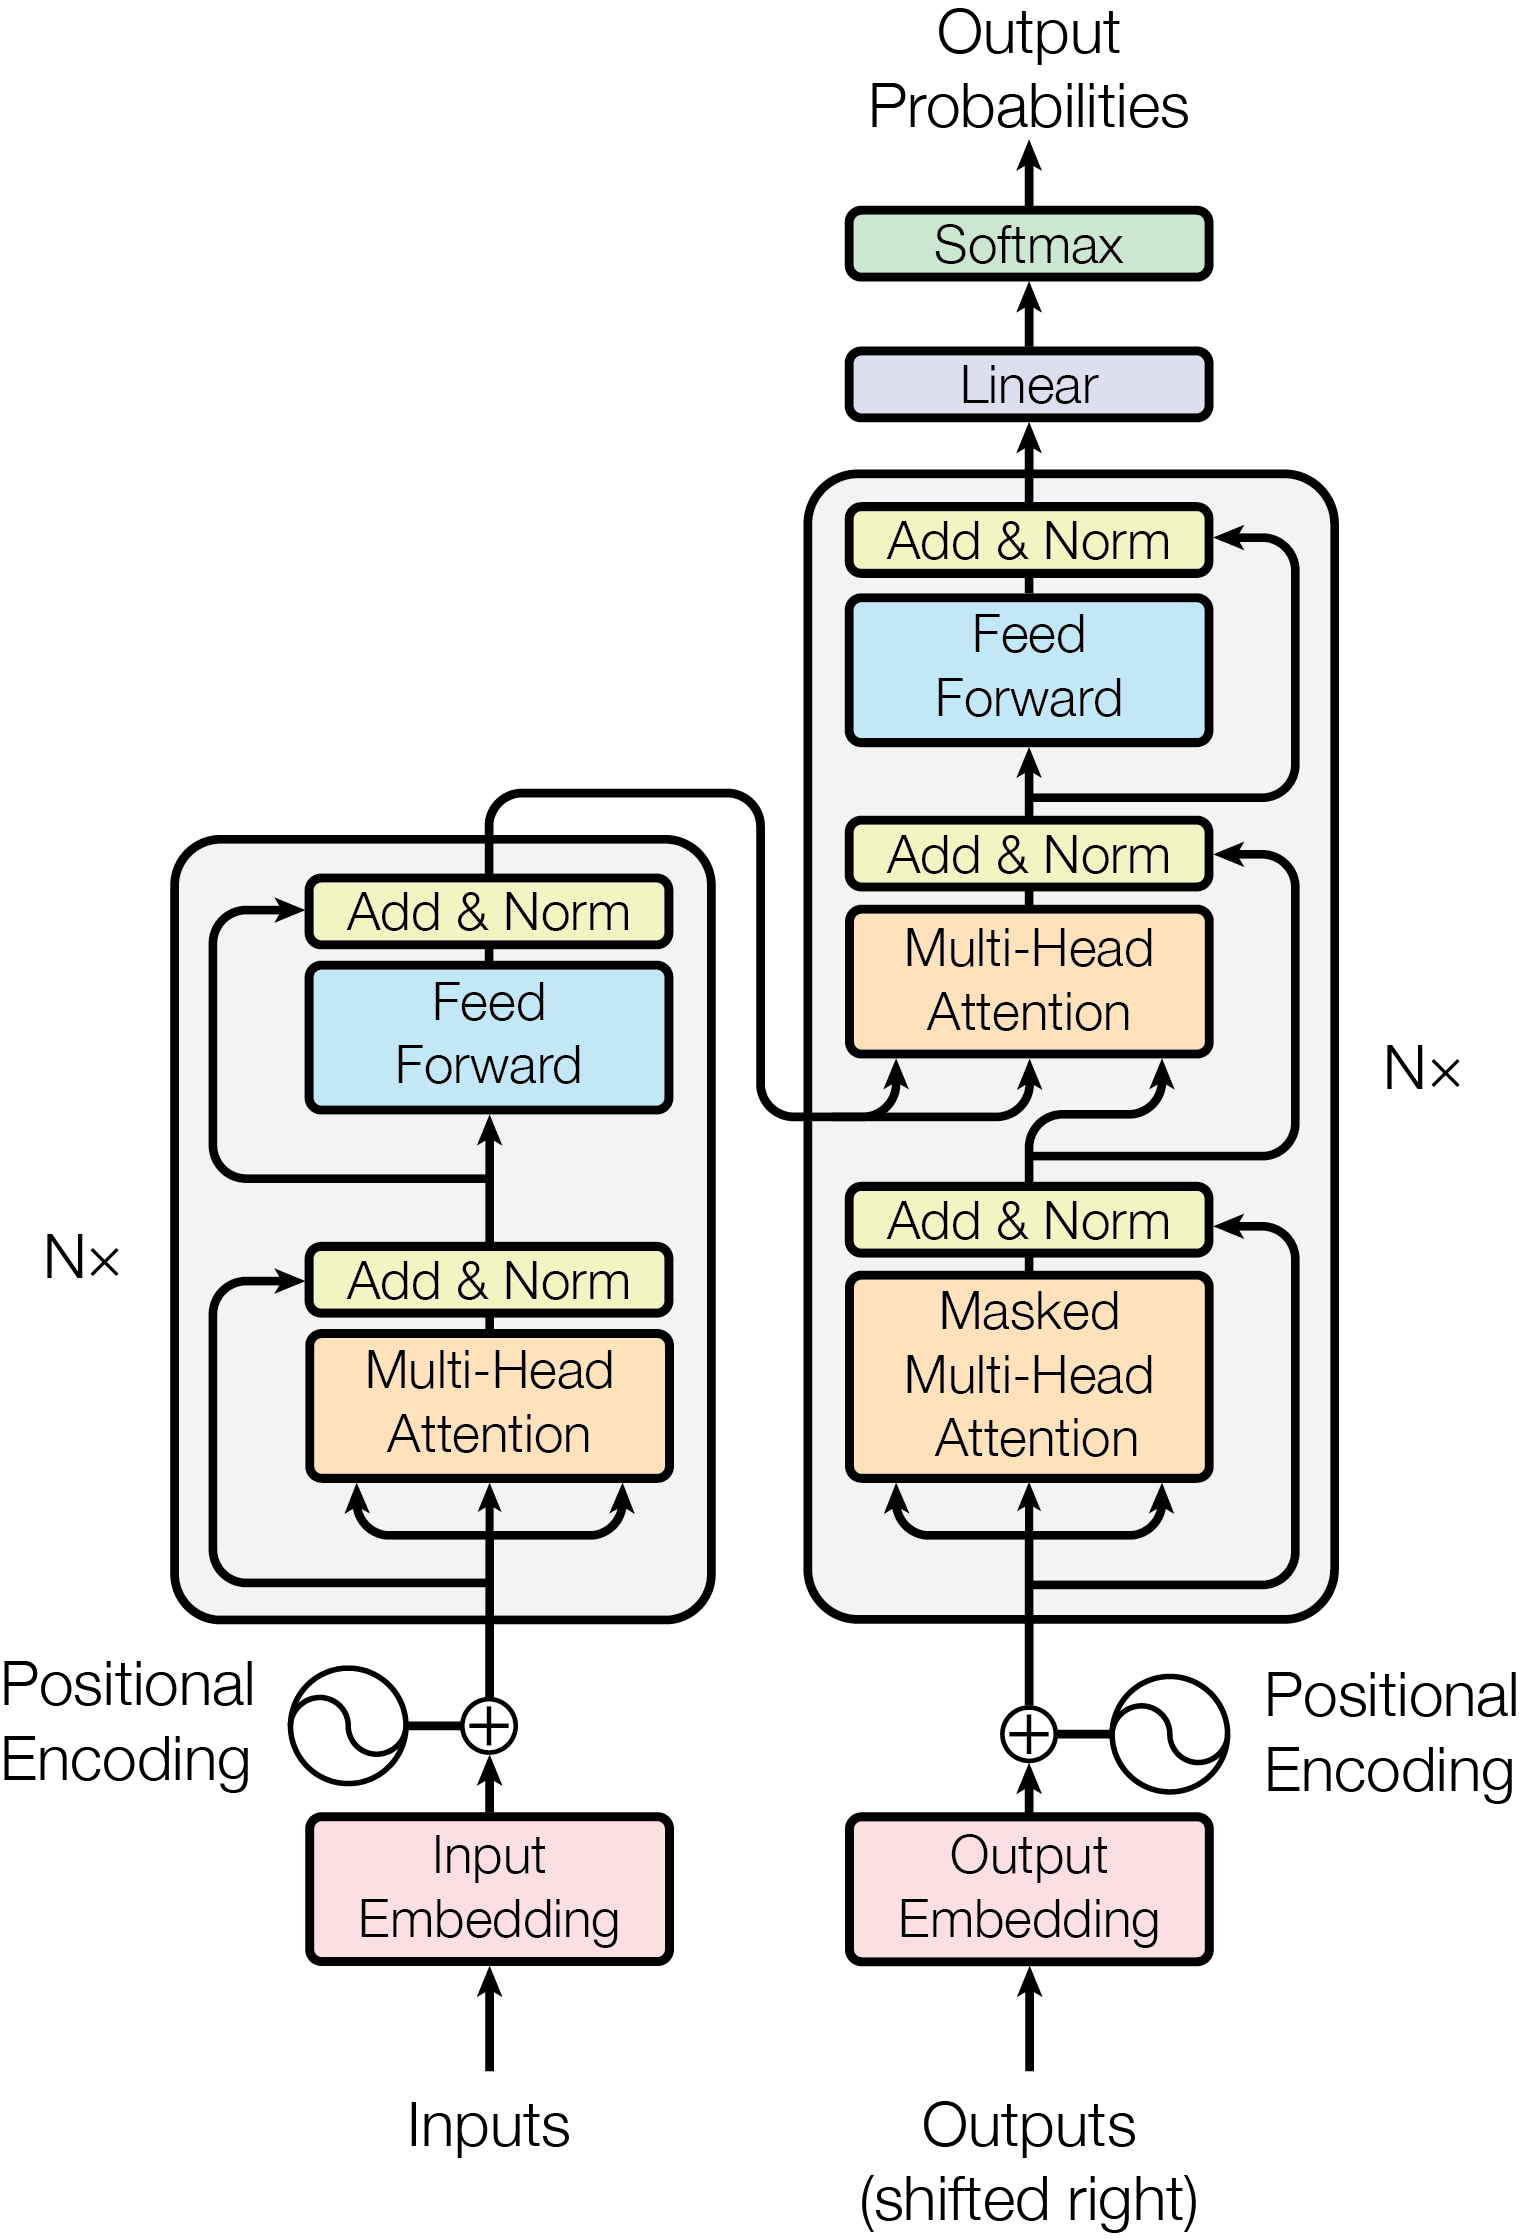
\includegraphics[scale=0.6]{paper_sources/attention_is_all_you_need/Figures/ModalNet-21}
    \caption{The Transformer - model architecture, \tiny{source: \cite{vaswani2017attention}}}
    \label{fig:model-arch}
\end{figure}

\subsubsection{Graphormer}
As an adaption of Transformers~\cite{vaswani2017attention} for graph representation learning, Graphormer~\cite{2021graphormer} was presented by Ying et al., providing a performant Transformer model, excelling in various graph representation learning tasks.

Graphormer achieves such good results by introducing three types of encodings to incorporate structural information of graphs in the feature vectors of nodes and edges.

To capture information about the importance of a node in a given network, Graphormer uses a measure called node centrality by utilizing degree centrality of a given node. This is done by introducing two new vectors for each node, one for the degree of ingoing edges and one for the outgoing ones. Those vectors are learnable scalars which are added to the node features, so node importance and semantic correlation are respected during self attention. \todo{\tiny add more information about learnable scalars, add general transforer structure to explain queries and keys}

The second encoding, called spatial encoding, is used to capture positional information for each node with respect to the network. This is achieved by using the distance of the shortest path between connected nodes and, once again, using a learnable scalar which is added as bias in the self-attention module. By doing that, the model can attend to a more relevant subset of the network according to the task. An example given in the paper is the possibility to increase attention to nodes surrounding a given node instead of nodes which lay further away.

Finally Graphormer introduces a method to include edge information in the model by adding an additional bias term to the attention module. This bias is created by averaging the dot-products of edge features and a learnable scalar of the edges describing the shortest path between each two connected nodes. \todo{\tiny perhaps add equations according to Transformer and Graphormer paper}

\subsubsection{GraphGPS}
L. Rampásek et al. introduced GraphGPS in their paper 'Recipe for a General, Powerful, Scalable Graph Transformer.'~\cite{2023graphgps} The objective of this model recipe is to provide a foundation for incorporating structural and positional information into node and edge features, while maintaining the flexibility of the model that implements these features.

GraphGPS serves as a preprocessor for the actual model learning on the dataset. The authors tested GraphGPS with several models, such as Transformer, Performer, BigBird, Gine, and more. They designed it to allow models that permit only Node Features, known as the Global Attention layer, as well as models that permit both Node and Edge Features, known as the MPNN layer. Both layers can also be used in combination to integrate the distinct advantages of two models.

The authors categorized structural and positional information into two types since the distance between nodes, although indicating the graph's structure, is insufficient to capture structural similarities. They incorporated this information by utilizing structural and positional encodings (SE and PE), which are divided into Local, Global, and Relative categories. Local and Global encodings are implemented as node features, while Relative encodings are implemented as edge features.

\subsubsection{Heterogeneous Interpolation on Graphs}
A winning entry for the dataset ogb-molpcba, called HIG-GraphClassification~\cite{tencenc2021Hig,tencenc2021HigPaper} was submitted to the OGB leaderboard in 2021 by Wang et al., providing an implementation and a brief technical report describing the research. By using their method combined with Graphormer, they were able to achieve better average precision than all previous submissions.

The report introduces heterogeneous interpolation, which is done by dropping the feature vectors of several randomly selected nodes and replacing them by the interpolated feature mix of all neighboring nodes.
By using a mixing ratio, the influence of each neighbors features can be adapted. To account for possible information loss, KL-Divergence constraint loss is added. By doing that, the distributions of two identical graphs remain similar after interpolating some feature vectors. The general idea was visualized by Wang et al. in \autoref{fig:hig_figure}.

\begin{figure}[h!]
    \centering
    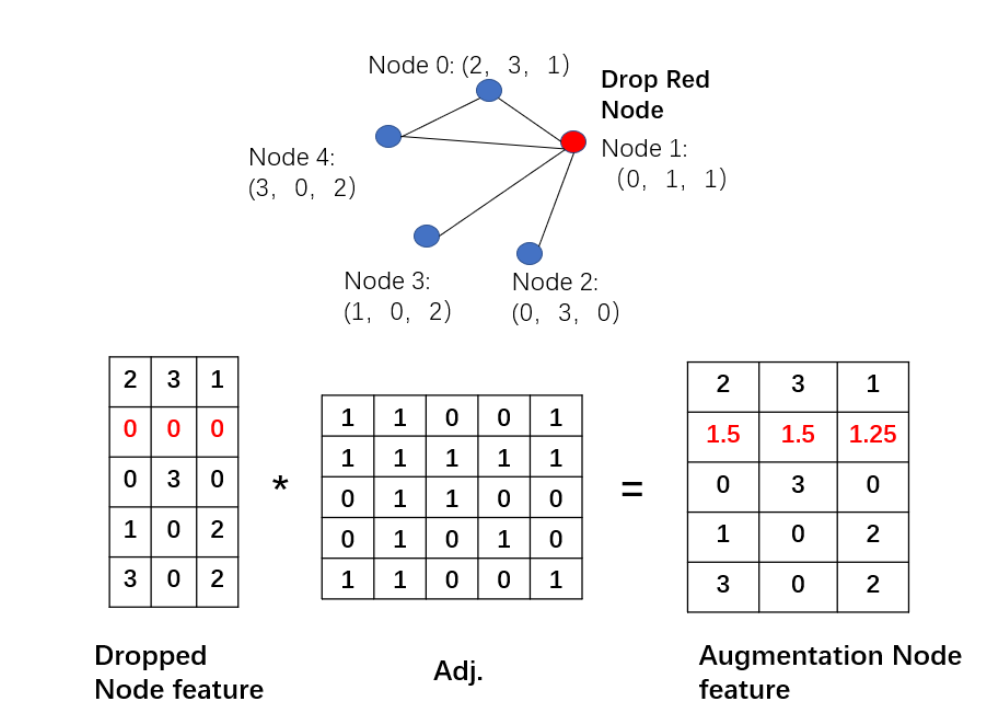
\includegraphics[scale=0.3]{tex/res/hig_figure.png}
    \caption{Visualization of HIG-GraphClassification by Wang et al., \tiny{source: \cite{tencenc2021HigPaper}}}
    \label{fig:hig_figure}
\end{figure}

We combine the idea of interpolating feature vectors of neighboring nodes with GraphGPS to test performance with different embedding methods.